\documentclass[letter]{article}
\usepackage[utf8]{inputenc}
\usepackage{amsmath}
\usepackage{graphicx}
\usepackage{caption}
\usepackage{subcaption}
\usepackage{listings}
\usepackage[top=1in, bottom=1in, left=1in, right=1in]{geometry}

%opening
\title{Fourier Transform Experimentation \\ Report}
\author{Luke Fraser}

\begin{document}

\maketitle

\begin{abstract}
In this assignment the use of the FFT (Fast Fourier Transofrm) is tested and analyzed to show its capabilties on different types of data. As well the theoretical aspects that were proven and understood in class are shown to appear in the experiemtnal results as well. The use of the Fourier Transform is far reaching and allows for a faster solution of the convolution in special cases. As well all of the experiments in this paper are implimented with the 1D FFT to show that a 2D FT can be computed through the use of a 1D FT.
\end{abstract}

\section{Experiment 1}
In this experiment we explore the use of the 1D FFT implementation provided in the ``fft.c'' code. The 1D FFT is an algorithm that performs a Descrete Fourier Transform (DFT). The FFT is an optimized implimentation of the DFT that has a running time O(NLog(N)).
\subsection{Part A}
Part A consists performing the FFT on a descrete function $f(x) = [1, 2, 4, 4]$. This preliminary experiment shows that we able to perfrom the FFT and return from the frequency domain and recover the original data set. In order to the use the FFT implimentation provided the data must be preprocessed in order to produce correct results. The data must first be supplied to the function as a one dimensional array of floating point values. The data must also start from position one in the array. This is contrary to standard ''C'' arrays which start at zero. As well the data must presented with its complex component inerleaved with the real component so that the structure of the array is as follows: $$[zero~position, real, imaginary, real, imaginary, real, ..., imaginary]$$ After the data is in the proper format to be fed to the FFT function the spektrum must be centered prior to performing the DFT so that a full period is in view in the result of the function. Good results were seen from the results of the FFT and the function $f(x)$ was able to go from the frequency domain and resturn with the same values.
\subsection{Part B}
Part B evalutaes the FT of a cosine function with a single frequency: $f(x) = cos(2 \pi u x / N)$. This function has 128 samples and cycles 8 times over the duration of the samples. The FT of the function is represented by two delta functions, one the reflection of the other across the y axis. The frequency of the function is 8 and the two delta functions are seen at positive 8 and negative 8 in the frequency domain. The value of the FT comes from the strength of the signal. This is the expected result from the FFT funtion. 
\subsection{Part C}
Part C shows the FT of the descrete reactangle function. This is an important FT to perform because it shows how the FT of a Rectangle function produces the sinc function in the frequency domain. In the case of this experiment the FFT is performed 128 samples of a Rect function. The function is represented as follows: $$f(x) = \left \{ \begin{array}{l l} 1 & \quad \text{if $33 \leq x \leq 96$}\\ 0 & \quad \text{Otherwise}\end{array} \right.$$
\section{Experiment 2}
In this experiment we impliment a 2D DFT from the 1D FFT used in the previous experiment. The 2D FFT is then used on different images to produce different 2D spektrums in the frequency domain. Tests are performed to see the issues of not shifting the spektrum to the center of the image. This experiment evaluates the importance of obtaining a full period in the frequency domain.
\subsection{Part A}
Part A uses a 2D function/image with a rectangle at the center of the image with a length and with of 32. The function is as follows: $$f(x,y) = \left \{ \begin{array}{l l} 1 & \quad \text{if $-16 < x \leq 16$ , $-16 < y \leq 16$}\\ 0 & \quad \text{Otherwise}\end{array} \right.$$

\begin{figure}[hbtp]
  \centering
  \begin{subfigure}{5.1cm}
    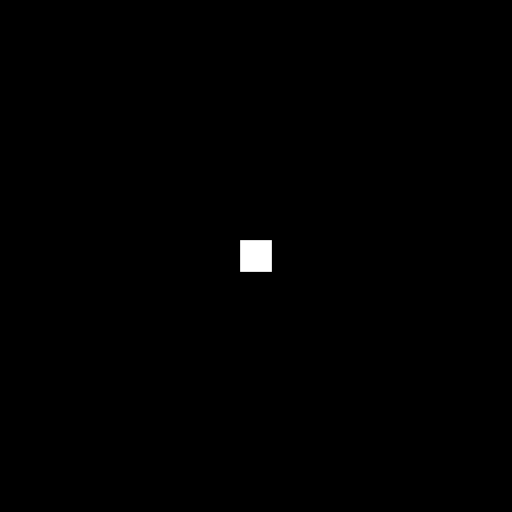
\includegraphics[width=5.1cm]{images/rect_512_32x32.png}
    \caption{Original Image.}
  \end{subfigure}
  \begin{subfigure}{5.1cm}
    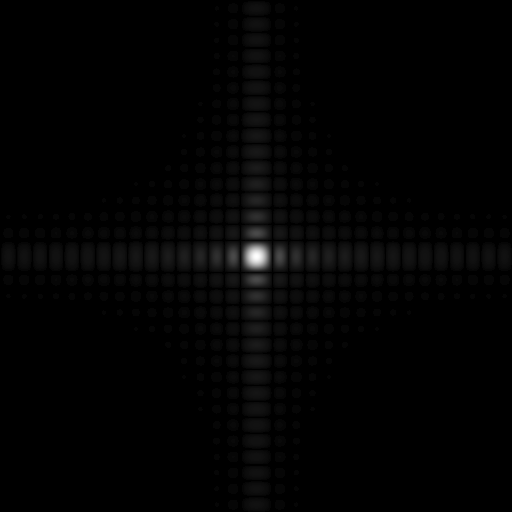
\includegraphics[width=5.1cm]{images/rect_512_32x32_FU_centered.png}
    \caption{Fourier transform centered.}
  \end{subfigure}
  \begin{subfigure}{5.1cm}
    
\includegraphics[width=5.1cm]{images/rect_512_32x32_FU.png}
    \caption{Fourier transform unentered.}
  \end{subfigure}
  \caption{Fourier transform of a 2D 32x32 rectangle function.}
  \label{fig:ft_3232}
\end{figure}
\subsection{Part B}
Part B uses a 2D function/image with a rectangle at the center of the image with a length and with of 64. The function is as follows: $$f(x,y) = \left \{ \begin{array}{l l} 1 & \quad \text{if $-32 < x \leq 32$ , $-32 < y \leq 32$}\\ 0 & \quad \text{Otherwise}\end{array} \right.$$

\begin{figure}[hbtp]
  \centering
  \begin{subfigure}{5.1cm}
    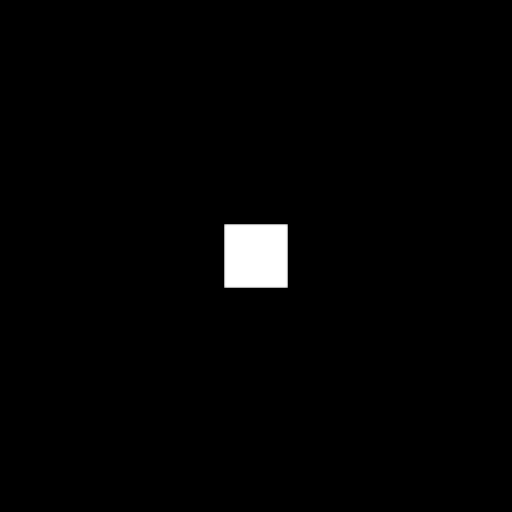
\includegraphics[width=5.1cm]{images/rect_512_64x64.png}
    \caption{Original Image.}
  \end{subfigure}
  \begin{subfigure}{5.1cm}
    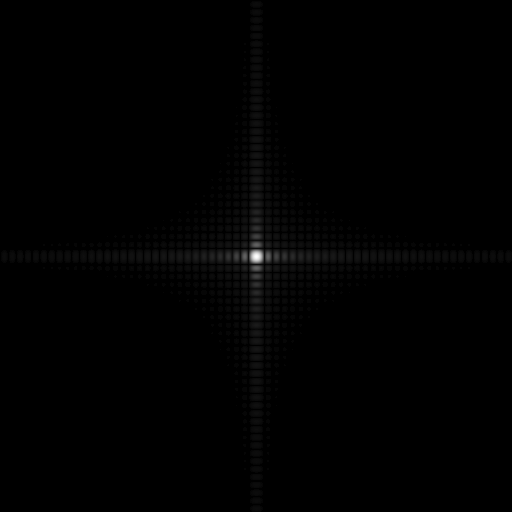
\includegraphics[width=5.1cm]{images/rect_512_64x64_FU_centered.png}
    \caption{Fourier transform centered.}
  \end{subfigure}
  \begin{subfigure}{5.1cm}
    
\includegraphics[width=5.1cm]{images/rect_512_64x64_FU.png}
    \caption{Fourier transform unentered.}
  \end{subfigure}
  \caption{Fourier transform of a 2D 64x64 rectangle function.}
  \label{fig:ft_6464}
\end{figure}
\subsection{Part C}
Part C uses a 2D function/image with a rectangle at the center of the image with a length and with of 128. The function is as follows: $$f(x,y) = \left \{ \begin{array}{l l} 1 & \quad \text{if $-64 < x \leq 64$ , $-64 < y \leq 64$}\\ 0 & \quad \text{Otherwise}\end{array} \right.$$

\begin{figure}[hbtp]
  \centering
  \begin{subfigure}{5.1cm}
    
\includegraphics[width=5.1cm]{images/rect_512_128x128.png}
    \caption{Original Image.}
  \end{subfigure}
  \begin{subfigure}{5.1cm}
    
\includegraphics[width=5.1cm]{images/rect_512_128x128_FU_centered.png}
    \caption{Fourier transform centered.}
  \end{subfigure}
  \begin{subfigure}{5.1cm}
    
\includegraphics[width=5.1cm]{images/rect_512_128x128_FU.png}
    \caption{Fourier transform unentered.}
  \end{subfigure}
  \caption{Fourier transform of a 2D 128x128 rectangle function.}
  \label{fig:ft_128128}
\end{figure}
\section{Experiment 3}
In this experiment we evaluate whether the magnitude or the phase component in the frequency is more important. To evaluate this we set either the phase component to zero or the magnitude to one to see the effects of the one in use over the other. The magnitude is set to one in order to remove its effects on the image while maintaining the a visual represntation of the image. This simply means that every frequency in the image will have the same magnitude.s
\subsection{Part A}
In part A the importance of the phase coponent is tested. The phase component in the frequency domain is set to zero prior to the inverse tranform.
\begin{figure}[hbtp]
  \centering
  \begin{subfigure}{5.1cm}
    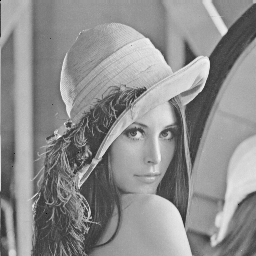
\includegraphics[width=5.1cm]{images/lenna.png}
    \caption{Original Image.}
  \end{subfigure}
  \begin{subfigure}{5.1cm}
    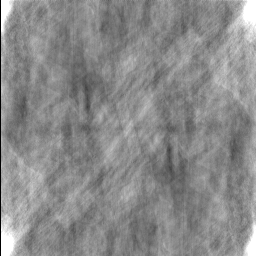
\includegraphics[width=5.1cm]{images/lenna_mag_only.png}
    \caption{No phase info.}
  \end{subfigure}
  \caption{Fourier Tranform where the phase information is set to zero and only the magnitude component is kept.}
  \label{fig:ft_mag}
\end{figure}
\subsection{Part B}
In part A the importance of the magnitude component is tested. The magnitude component in the frequency domain is set to one prior to the inverse tranform.

\begin{figure}[hbtp]
  \centering
  \begin{subfigure}{5.1cm}
    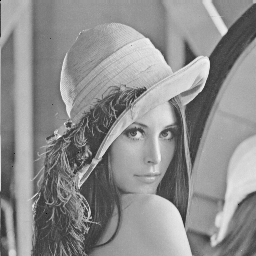
\includegraphics[width=5.1cm]{images/lenna.png}
    \caption{Original Image.}
  \end{subfigure}
  \begin{subfigure}{5.1cm}
    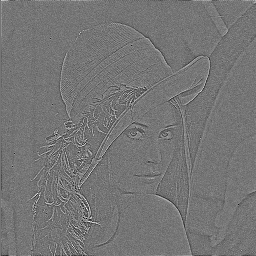
\includegraphics[width=5.1cm]{images/lenna_phase_only.png}
    \caption{No magnitude info.}
  \end{subfigure}
  \caption{Fourier Tranform where the magnitude information is set to onq and only the phase component is kept.}
  \label{fig:ft_phase}
\end{figure}

\end{document}
